% 1977 年江苏南京市初试卷第六题：圆 O 中直径 AB 与弦 AC 的夹角 15°，过 C 的切线交 AB 延长线于 P，OP=24cm（按源卷第 2 页布局；r=2，OP=2/\cos30°≈2.309，P 在 B 右侧）
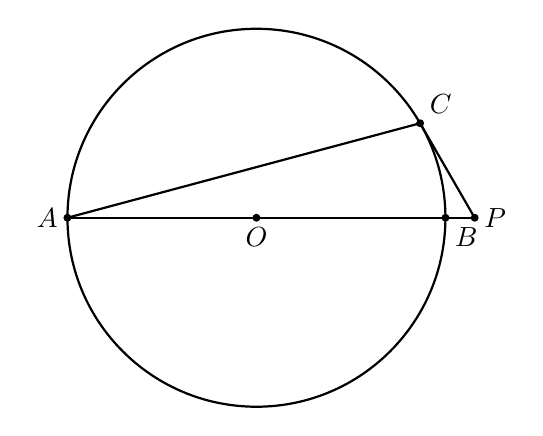
\begin{tikzpicture}[scale=1.2]
  \coordinate (O) at (0,0);
  \coordinate (A) at (-2,0);
  \coordinate (B) at (2,0);
  \coordinate (C) at (1.732,1);
  \coordinate (P) at (2.309,0);
  \draw[thick] (O) circle (2);
  \draw[thick] (A)--(P);
  \draw[thick] (A)--(C);
  \draw[thick] (C)--(P);
  \fill (O) circle (1.2pt) node[below] {$O$};
  \fill (A) circle (1.2pt) node[left] {$A$};
  \fill (B) circle (1.2pt) node[below right] {$B$};
  \fill (C) circle (1.2pt) node[above right] {$C$};
  \fill (P) circle (1.2pt) node[right] {$P$};
\end{tikzpicture}
